% VUT FIT MITAI
% MSZ 2021/2022
% Author: Vladimir Dusek
% Login: xdusek27

%%%%%%%%%%%%%%%%%%%%%%%%%%%%%%%%%%%%%%%%%%%%%%%%%%%%%%%%%%%%%%%%%%%%%%%%%%%%%%%%

% Path to figures
\graphicspath{{upa/prostorove_db/figures}}

%%%%%%%%%%%%%%%%%%%%%%%%%%%%%%%%%%%%%%%%%%%%%%%%%%%%%%%%%%%%%%%%%%%%%%%%%%%%%%%%

\chapter{UPA~--~Prostorové DB (problematika mapování prostoru, ukládání, indexace; využití).}

%%%%%%%%%%%%%%%%%%%%%%%%%%%%%%%%%%%%%%%%%%%%%%%%%%%%%%%%%%%%%%%%%%%%%%%%%%%%%%%%

\section{Zdroje}

\begin{compactitem}
    \item \path{PDB-Spatial-CZ.pdf}
    \item \path{03-spatial_databases.pdf}
    \item \path{szz-kastak.pdf}
    \item \path{szz-discord-bazi.pdf}
\end{compactitem}

%%%%%%%%%%%%%%%%%%%%%%%%%%%%%%%%%%%%%%%%%%%%%%%%%%%%%%%%%%%%%%%%%%%%%%%%%%%%%%%%

\section{Úvod a kontext}

\begin{compactitem}
    \item Prostorové databáze podporují ukládání, zpracování a manipulace s prostorovými daty.

    \item Jsou případem pokročilého databázového systému -- postrelačního databázového systému.

    \item Jsou schopné spravovat data, která se váží k určitému (libovolně velikému) prostoru. Mají schopnost spravovat velké množství relativně jednoduchých geometrických objektů.

    \item Jejich DDL (\textit{data definition language}) a DML (\textit{data manipulation language}) zahrnují prostorové datové typy. Ty jsou podpořeny i na implementační úrovni, takže je možné efektivně provádět operace indexace, vyhledávání, spojování (join), \dots

    \item Jako uživatelé ukládáme geometrické (základní matematicko-geometrické tvary reprezentující např. města, řeky, domy, atomy, planety) a topologické údaje (vzájemné vztahy mezi ukládanými objekty, jako např. vzdálenost). \begin{compactitem}
        \item Popisujeme entity v prostoru a prostor jako takový.
        \item V rámci geometrických údajů mluvíme o entitách jako bod, lomená čára, (vyplněný) polygon.
    \end{compactitem}
\end{compactitem}

%%%%%%%%%%%%%%%%%%%%%%%%%%%%%%%%%%%%%%%%%%%%%%%%%%%%%%%%%%%%%%%%%%%%%%%%%%%%%%%%

\section{Problémy a jejich řešení}

\begin{compactitem}
    \item Obvykle uvažujeme dvou až tří rozměrný euklidovský prostor, který je spojitý ve svých dimenzích a pozice každého bodu je definována uspořádanou uspořádanou $n$-ticí $p \in \mathbb{R}^n$.

    \item Pro vzdálenost bodů v $n$ rozměrném prostoru platí euklidovská metrika:
    $$ d(A, B) = \sqrt{(a_1 - b_1)^2 + \ldots + (a_n - b_n)^2} $$

    \item Problém, který nastává, je nemožnost počítače reprezentovat přesně reálná čísla -- dochází k diskretizaci prostoru. \begin{compactitem}
        \item Tento problém vyvstává např. při výpočtu průsečíku, či sousednosti.
    \end{compactitem}
    \begin{figure}[H]
        \centering
        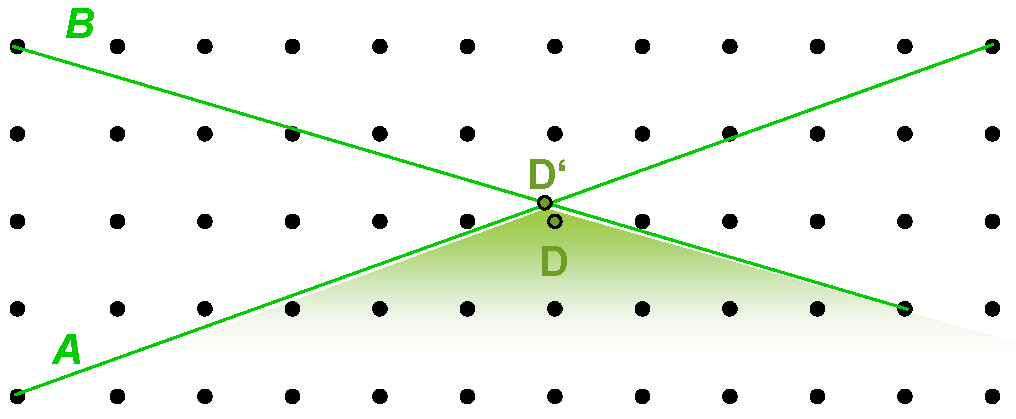
\includegraphics[width=0.75\linewidth]{spatial-problem.pdf}
        \caption{Problém diskretizace (spojitého) prostoru při reprezentaci průsečíku dvou úseček.}
    \end{figure}

    \item Řešením je oddělení typů a operací nad prostorovými daty, tak aby byl korektně ošetřen tento číselný problém vzhledem ke geometrickému systému. Lze použít simplexy nebo úplné deskriptory (realms).
\end{compactitem}

\subsection{Simplexy}

\begin{compactitem}
    \item Simplexy jsou nejmenší nevyplněné objekty daného rozměru.
    \item Použijeme jednoduché geometrické entity ke skládání složitějších celků.
    \begin{figure}[H]
        \centering
        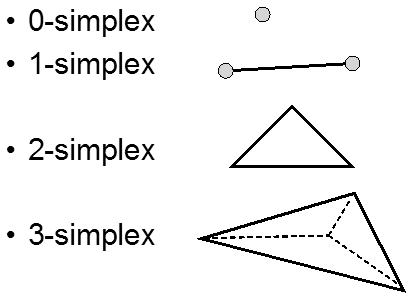
\includegraphics[width=0.35\linewidth]{simplexy.png}
        \caption{Simplexy.}
    \end{figure}
    \item Lze vypozorovat, že $d$-simplex sestává z $d+1$ simplexů rozměru $d-1$.
    \item Takové tvořící elementy se potom nazývají styky (faces).
    \item Kombinace simplexů do složitějších struktur je povolena jen tehdy, pokud průnik libovolných dvou simplexů je styk.
    \item Wikipedie: Simplex (či n-simplex) je n-rozměrným zobecněním trojúhelníku. Jedná se o konvexní obal množiny $n+1$ afinně nezávislých bodů umístěný v euklidovském prostoru dimenze $n$ či vyšší.
\end{compactitem}

\subsection{Úplné popisy (deskriptory, \textit{realms})}

\begin{compactitem}
    \item Souhrnný popis všech objektů v databázi.
    \item Formálněji je to množina bodů, úseček, případně vyšších celků, nad sítí bodů, které mají tyto vlastnosti: \begin{compactitem}
        \item každý (koncový) bod je bodem sítě;
        \item každý koncový bod usečky (složitějšího útvaru) je bodem sítě;
        \item žádný vnitřní bod úsečky (složitějšího útvaru) není zaznamenán v síti;
        \item žádné dvě úsečky (složitější útvary) nemají ani průsečík ani se nepřekrývají.
    \end{compactitem}
\end{compactitem}

%%%%%%%%%%%%%%%%%%%%%%%%%%%%%%%%%%%%%%%%%%%%%%%%%%%%%%%%%%%%%%%%%%%%%%%%%%%%%%%%

\section{Mapování reality}

\begin{compactitem}
    \item Při popisu reality musíme být schopni definovat vnořené objekty (např. plochu uvnitř plochy). To realizujeme pomocí R-cyklů a R-ploch.
\end{compactitem}

\subsection{R-cyklus}

\begin{compactitem}
    \item R-cyklus je polygon (mnohoúhelník) uložený v diskrétní prostorové reprezentaci.

    \item Tj. uzavřená lomená úsečka, která je vytvořena podle pravidel ukládání deskriptorů. \begin{compactitem}
        \item Skládá se z posloupností $n$ úseček $s_1, \ldots, s_n$ a pro každou úsečku musí platit, že koncový bod úsečky $s_i$ je roven počátečnímu bodu úsečky ${\displaystyle s_{(i+1)\mod{n}}}$.

        \item Navíc žádné dvě úsečky $s_i$, $s_j$, kde $i, j \in {1, \ldots, n}$ se nemohou protínat.
    \end{compactitem}
\end{compactitem}

\begin{figure}[H]
    \centering
    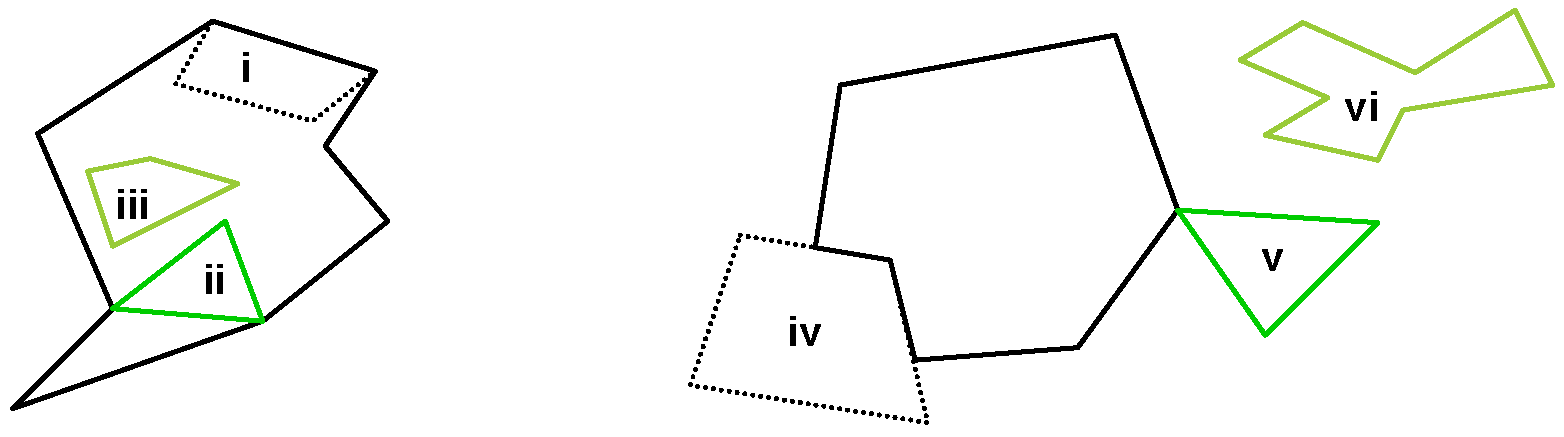
\includegraphics[width=1\linewidth]{r_loop.pdf}
    \caption{Různé míry vnoření polygonů (plošně -- i, ii, iii, hranově -- ii, iii, zcela/vrcholově -- iii) a disjunkce polygonů (plošně -- iv, v, vi, hranově -- vi, v, zcela/vrcholově -- vi).}
\end{figure}

\subsection{R-plocha}

\begin{compactitem}
    \item Jak vložit několik poligonů do jednoho? \begin{compactitem}
        \item Máme r-cyklus a uvnitř něho další r-cykly.
    \end{compactitem}

    \item R-plocha $f$ je dvojice $f = (c, H)$, kde je $c$ je R-cyklus a $H$ je množina R-cyklů, s jistými vlastnostmi: \begin{compactitem}
        \item $ \forall h \in H $ je hranově vnořený v $c$;
        \item $ \forall h_i, h_j \in H : h_i \not= h_j$ platí, že $h_i$ a $h_j$ jsou hranově disjunktní;
        \item není možné vytvořit žádný další R-cyklus ze segmentů popisujících R-plochu $f$.
    \end{compactitem}

\end{compactitem}

\subsection{Vnořená R-plocha}

\begin{compactitem}
    \item Nechť $f = (f_0, F)$ a $g = (g_0, G)$ jsou dvě R-plochy. Řekneme, že $f$ je plošně vnořená v $g$ právě tehdy když: \begin{compactitem}
        \item $f_0$ je plošně vnořená v $g_0$ a zároveň;
        \item $\forall g \in G : g$ je plošně disjunktní s $f_0$ a nebo $\exists f \in F : g$ je plošně vnořené v $f$.
    \end{compactitem}
\end{compactitem}

\begin{figure}[H]
    \centering
    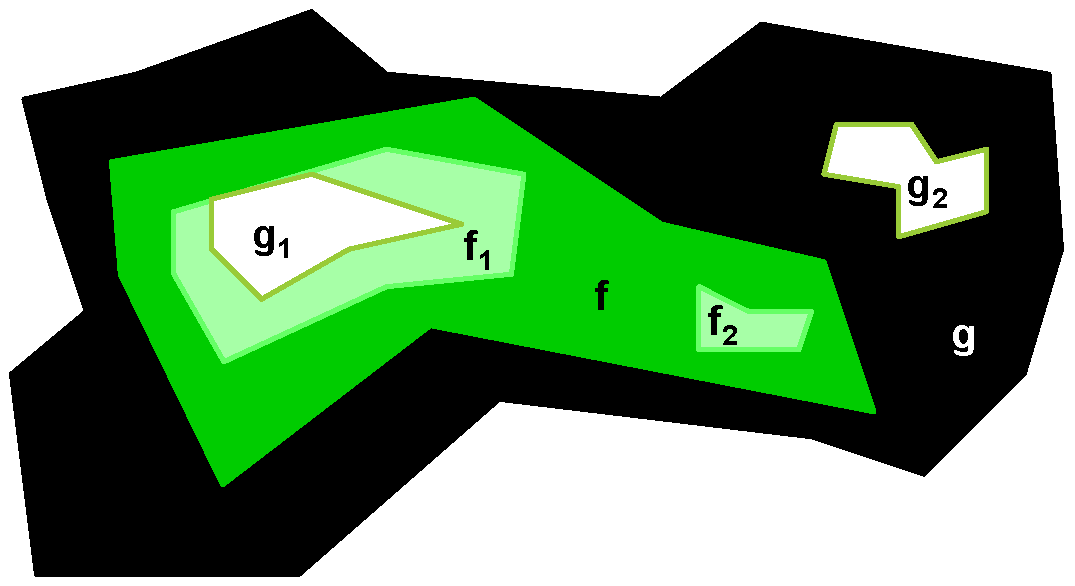
\includegraphics[width=0.75\linewidth]{r_area.pdf}
    \caption{R-plochy $f$ je vnořená v $g$.}
\end{figure}

\subsection{Region}

\begin{compactitem}
    \item Množina hranově disjunktní R-ploch.
\end{compactitem}

\subsection{Vnořený region}

\begin{compactitem}
    \item Nechť $R, G$ jsou regiony, potom F je plošně vnořený v G právě tehdy když
    $$ \forall f \in F : \exists g \in G : f \text{ je plošně vnořená v } g $$
\end{compactitem}

%%%%%%%%%%%%%%%%%%%%%%%%%%%%%%%%%%%%%%%%%%%%%%%%%%%%%%%%%%%%%%%%%%%%%%%%%%%%%%%%

\section{Operace nad prostorovými datami}

\begin{compactitem}
    \item Číselné konstanty/charakteristiky (vypočítané při ukládání, tedy při operacích):\break délka, velikost, objem, plocha, průměr, obvod, \ldots

    \item Prostorové konstanty/charakteristiky (počítají se během ukládání, vytvářejí nové prostorové konstanty/charakteristiky)
    hodnotu: střed, těžiště, \ldots

    \item Metriky (číslo jako výsledek, nelze vypočítat předem): vzdálenost, průměr pro množinu prvků, \ldots

    \item Predikáty: stejné, uvnitř, protíná, sousedí, \ldots

    \item Vytvářejí se/vybírají se nové objekty: průsečík, rozdíl, voronoi, konvexní trup, \ldots
\end{compactitem}

%%%%%%%%%%%%%%%%%%%%%%%%%%%%%%%%%%%%%%%%%%%%%%%%%%%%%%%%%%%%%%%%%%%%%%%%%%%%%%%%

\section{Ukládání dat}

\begin{compactitem}
    \item Prostorové databáze si musí umět poradit s různorodou velikostí dat, kde datové položky se mohou pro hodnoty jednoho typu významně lišit a nabývat vysokých hodnot.

    \item Způsob uložení je konzistentní pro různou velikost dat. \begin{compactitem}
        \item Pro každá prostorová data tak dojde k vyčlenění dat, které se nemění s charakterem vkládaného objektu.
        \item Ostatní data se ukládají mimo, do zvláštních datových stránek, které tak leží mimo a nebrání rychlému zpracování.
    \end{compactitem}

    \item Pokud prostorová data nepřekročí určitou velikost, tak jsou uložena stejně, jako ostatní. V rámci jedné stránky na disku/v paměti je možné mít více datových záznamů, jakmile však délka přeroste jistou mez, tak je uložen odkaz na souvislou oblast na disku, kde jsou velká data uložena za sebou.

    \item Velké data (cykly, plochy, regiony, \ldots) se neukládají jako běžná data -- v tabulce je pouze ukazatel.

    \item V některých případech se volí předzpracování prostorových dat -- ukládají se např. výsledky agregačních funkcí (průměr, suma, střed) nebo prvotní aproximace.

    \item Bývají uložené předpočítané hodnoty (délky, obsahy, objemy, \ldots) a aproximace. Např. průsečíky se nepočítají při dotazu, ale jsou předpočítané a uložené v prostorových objektech.
\end{compactitem}
